\documentclass[12pt]{article}
\usepackage[utf8]{inputenc}
\usepackage{csquotes, amsmath, amssymb, graphicx, tikz, geometry, multicol}
\usepackage{wrapfig}
\geometry{margin=1in}

\setlength{\parindent}{0in}

\begin{document}

\begin{titlepage}

\begin{center}
    \Huge{Astronomy class 1: Elliptic orbits and celestial mechanics}
    
    \vspace{1in}
    
    \Large{Simon Wu}
    
    \Large{April 11, 2021}
    
    \vspace{1in}
    
    \Large{Olympiads School - Mr. Horbatsch}

    
\end{center}

\tableofcontents

\end{titlepage}

\section{Course overview}

\subsection{Textbook section}

The textbook that we are using in this course is \emph{Introduction to Astronomy} by \emph{Dr. Karina Kjaer}.
This class was based on material from \emph{Chapter 1} of the textbook.

\subsection{Fundamental theories of astronomy}

Astronomy is understanding things in our night sky.
To this end, we use two major theories: \emph{gravity} and \emph{quantum mechanics}.

\subsubsection{Gravity}

\begin{wrapfigure}{r}{0.2\textwidth}
    \centering
    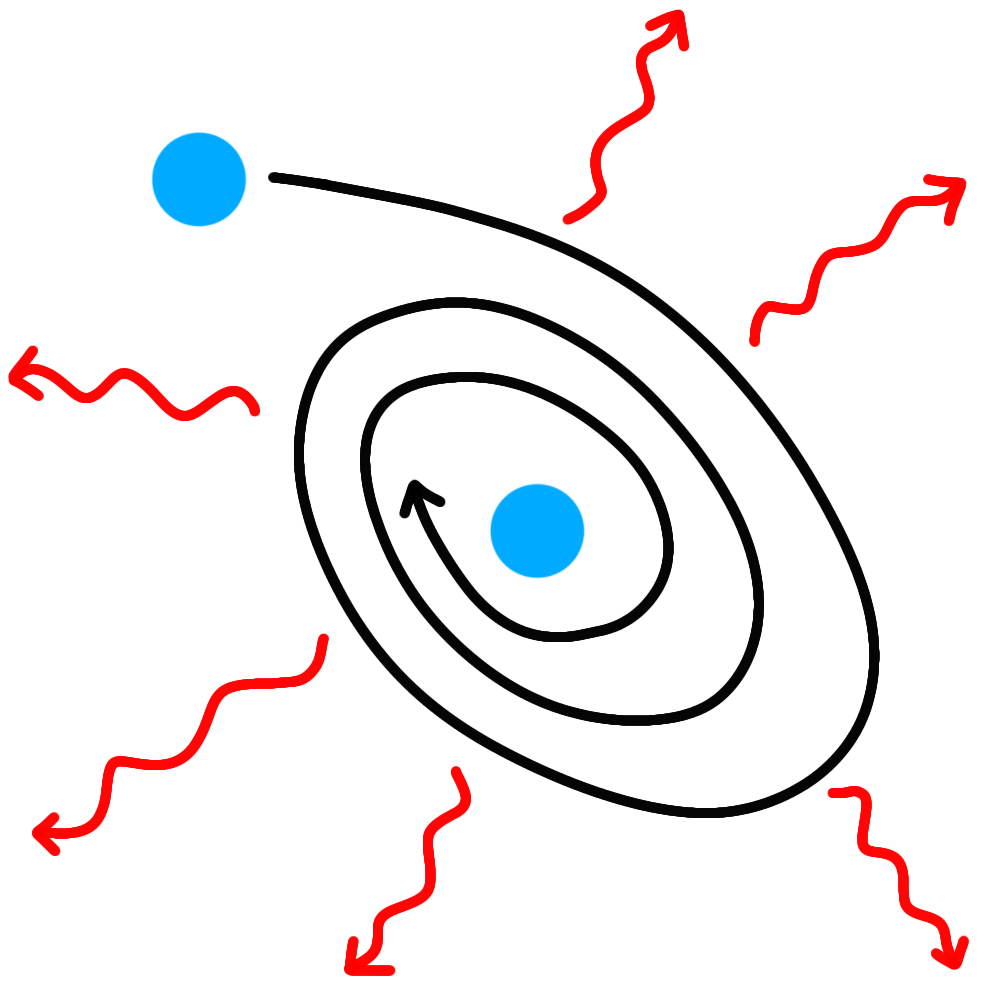
\includegraphics[width=0.2\textwidth]{binary_pulsar}
    \label{fig:binarypulsar}
    \caption{Binary pulsar diagram.}
\end{wrapfigure}

Gravity is used to explain how objects in the night sky move.
In general, there is \emph{Newtonian gravity} (from Isaac Newton in the 1600's), and \emph{general relativity} (from Albert Einstein in the early 1900's).

Newtonian gravity is good for most things in the night sky.
However, not everything is that simple: some phenomena require the use of general relativity to accurately describe and explain.
General relativity is generally required for:
	
\begin{itemize}
	\item Black holes
	\item Cosmology (understanding the evolution of the entire universe)
	\item Binary pulsars (Figure \ref{fig:binarypulsar})
	\begin{itemize}
		\item Their orbits are shrinking ellipses and create spirals
		\item The effect requires general relativity to understand
		\begin{itemize}
			\item They output \emph{gravitational radiation} and lose energy in their orbits
		\end{itemize}
	\end{itemize}
	\item The orbit of Mercury (when high precision is needed)
	\begin{itemize}
		\item This is because Mercury is the planet closest to the Sun
		\item If you only need decent accuracy ($\sim 1\%$) then Newtonian gravity is sufficient
	\end{itemize}
\end{itemize}


\subsubsection{Quantum mechanics}

Quantum mechanics is mostly used to explain how stars shine (e.g. how the Sun shines).
It can predict the properties of emitted light from various atoms, and is also required to explain things like the stability of neutron stars and white dwarfs.

\newpage

\subsection{Length scales}

\begin{itemize}
	\item $10^{-15}$ meters: size of individual protons/neutrons.
	\item $10^{-10}$ meters: size of individual atoms.
	\item $1$ meter: normal stuff.
	\item $1$ AU, $10^{11}$ meters: the astronomical unit (AU), which is the Earth-Sun distance.
	\item $1$ pc, $1$ ly, $10^{16}$ meters: a light year (ly), parsec (pc, or parallax arc-second). About the distance to the nearest star, $\alpha$-Centauri
	\item $1$ kpc, $10^{19}$ meters: a kiloparsec. Magnitude of the size of galaxies e.g. Andromeda.
	\item $1$ Mpc, $10^{22}$ meters: a megaparsec. About the size of universe clusters.
	\item $1$ Gpc, $10^{25}$ meters: a gigaparsec. About the size of the observable universe. 
\end{itemize}

\section{Circular orbits}

\begin{wrapfigure}{r}{0.5\textwidth}
    \centering
    
\includegraphics[width=0.5\textwidth]{circular_orbit}
    \label{fig:circularorbit}
    \caption{Circular orbit diagram.}
\end{wrapfigure}

Circular orbits can be parametrized as follows:

\[
x(t) = r\cos(\omega t)
\]

\[
y(t) = r\sin(\omega t)
\]

Of course, $v = r\omega$.
If the mass $M$ is considered to be much larger than $m$, the following equations can be derived for the orbital velocity:

\[
F_{net} = m\frac{v^2}{r} = \frac{GmM}{r^2}
\]

\[
v^2 = \frac{GM}{r}
\]

\newpage

\section{Elliptic orbits}

\subsection{Ellipse equation}

\begin{figure}[h]
    \centering
    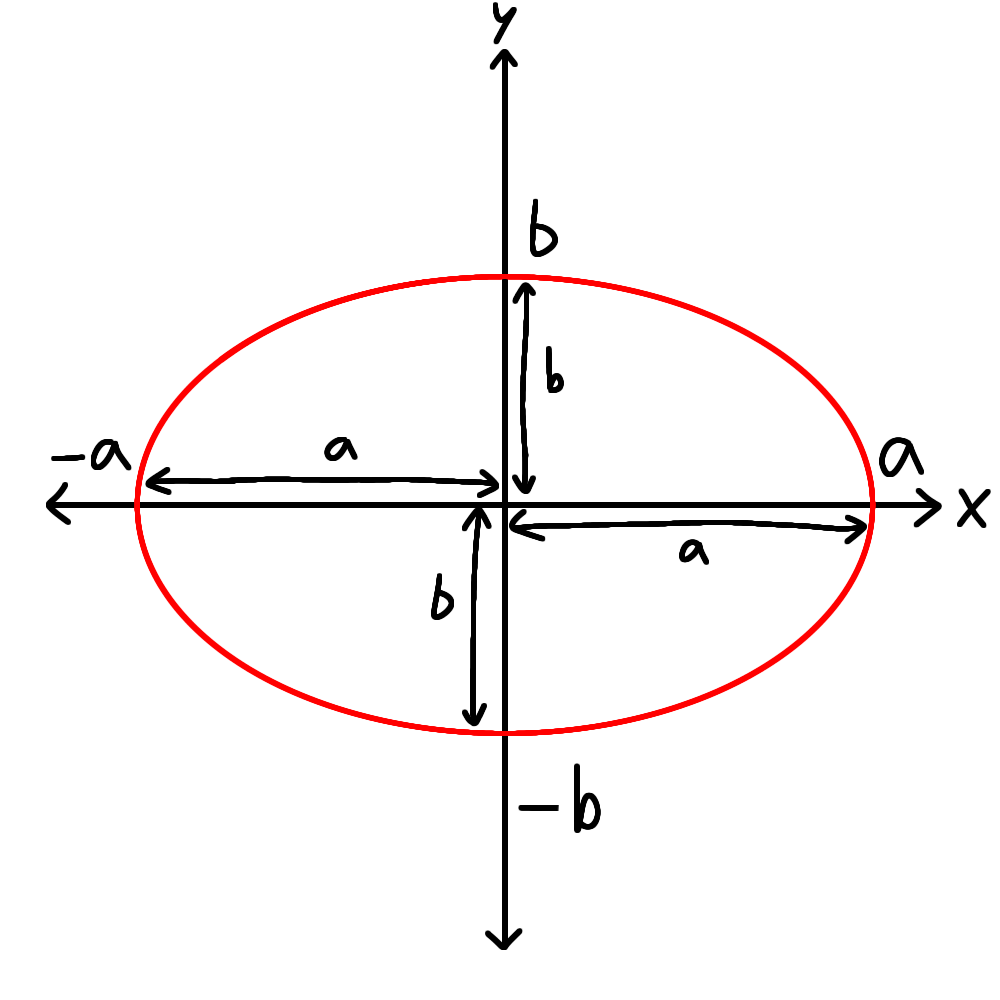
\includegraphics[width=0.5\textwidth]{ellipse_equation}
    \label{fig:ellipseequation}
    \caption{Ellipse graph.}
\end{figure}

An ellipse can be defined with the following equation:

\[
\frac{x^2}{a^2} + \frac{y^2}{b^2} = 1
\]

Take $a,b>0$ and $a \geq b$.
$a$ is called the \emph{semi-major axis}, and $b$ is called the \emph{semi-minor axis}.
Notice that if $a = b$, it simplifies to a circle ($x^2 + y^2 = a^2$), of radius $a$.

\subsubsection{Eccentricity}

The eccentricity of an ellipse is represented with $\epsilon$.

\[
\epsilon = \sqrt{1 - b^2 / a^2} \in \mathbb{R}
\]

$b^2 / a^2 \leq 1$, so $0 \leq \epsilon \leq 1$.
Notice:

\begin{itemize}
	\item When $\epsilon = 0$, $b/a = 1$, and the ellipse reduces to a circle.
	\item When $\epsilon = 1$, $b/a = 0 \longrightarrow \lim_{b \to 0}$, and the ellipse collapses to a straight line segment.
\end{itemize}

\newpage

\subsection{Naive parametrization of elliptic orbit}

Knowing the parametrization of an ellipse, there is an immediate parametrization that you may try to represent an elliptical orbit.

\[
x(t) = a\cos(\omega t)\text{, }y(t) = b\sin(\omega t) \longrightarrow \frac{[x(t)]^2}{a^2} + \frac{[y(t)]^2}{b^2} = 1
\]

However, this while this parametrization \emph{does} represent a particle moving on an elliptic path, it does \emph{not} represent
the motion of an object orbiting another.
This is because the \emph{speed} of the orbiting object is not properly represented.

\subsubsection{Speed of object in this parametrization}

\begin{figure}[h]
    \centering
    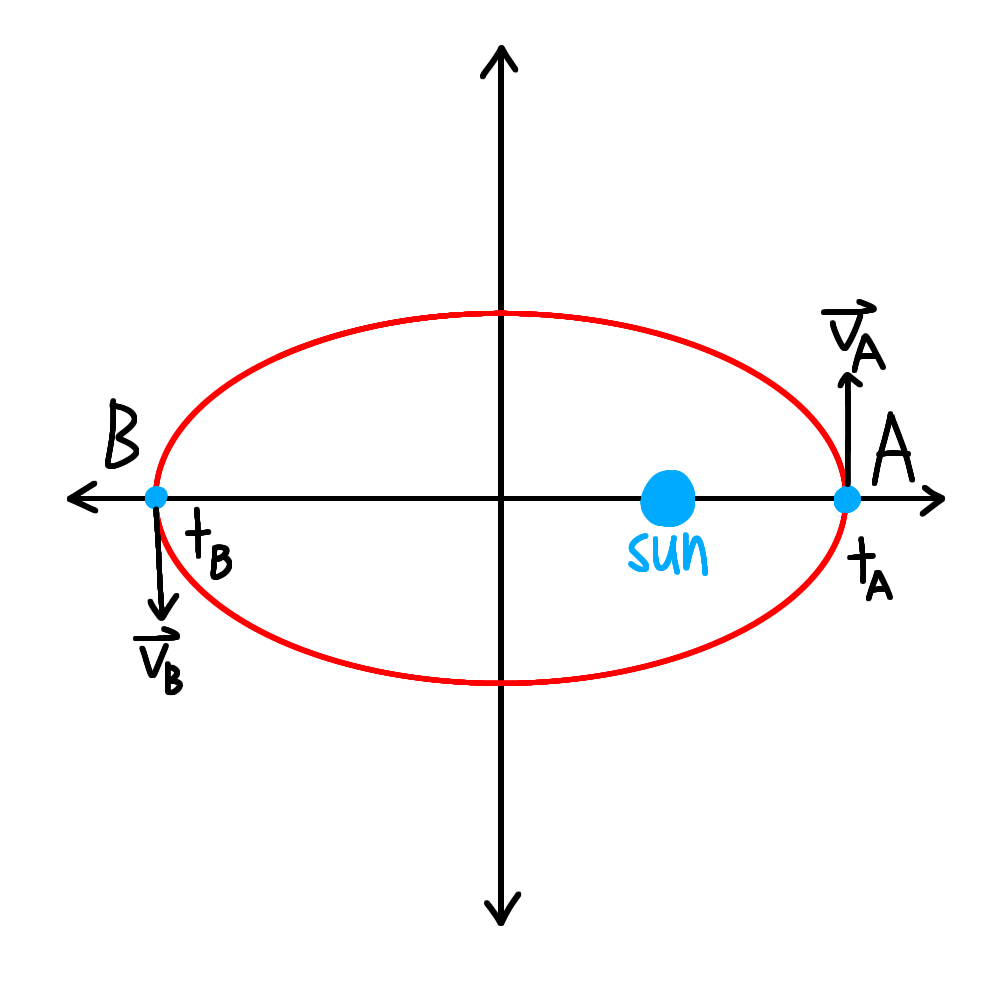
\includegraphics[width=0.5\textwidth]{elliptic_orbit}
    \label{fig:ellipticorbit}
    \caption{Elliptic orbit diagram.}
\end{figure}

Knowing that the orbital period $T$ is $2\pi / \omega$, let $t_A = 0$ and $t_B = \pi / \omega$ (halfway through the orbit).

\[
\dot{x}(t) = -a\omega \sin(\omega t)\text{, }\dot{y}(t) = b\omega \cos(\omega t)
\]

\[
\left| \vec{v}(t) \right| = \sqrt{a^2 \omega^2 \sin^2(\omega t) + b^2 \omega^2 \cos^2(\omega t)}
\]

\[
\left| \vec{v}(t_A) \right| = \left| \vec{v}(0) \right| = b\omega \text{, } \left| \vec{v}(t_B) \right| = \left| \vec{v}(\pi / \omega) \right| = b\omega\text{, } \left| \vec{v}(t_A) \right| =\left| \vec{v}(t_B) \right| 
\]

As can be observed in the equations, with this parametrization, the speed of the orbiting object at $A$ is the same as its speed at $B$: however, in real life, speeds at those locations will vary a lot!
In actuality, there really is no simple equation or expression for $x(t)$, $y(t)$, or even $r(t)$ and $\theta (t)$!

\newpage

\subsection{Properties of an elliptic orbit}

Given a mass $m$ orbiting a mass $M$, with mass $M >> m$, $M$ can be modelled as being fixed to the original of an inertial reference frame (essentially modelled as being at rest).

\begin{figure}[h]
    \centering
    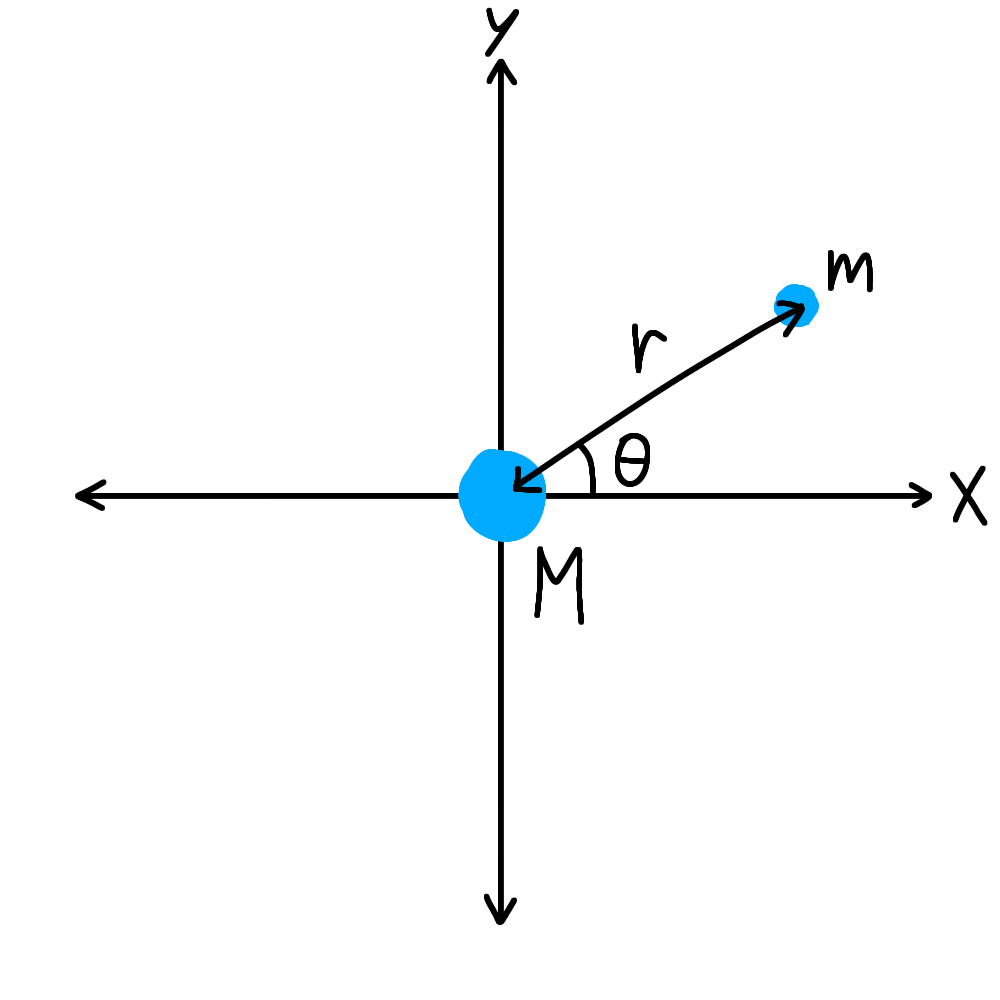
\includegraphics[width=0.5\textwidth]{polar_coord}
    \label{fig:polarcoord}
    \caption{Diagram of situation representing elliptic orbit.}
\end{figure}

To understand the motion of the mass $m$ in orbit around $M$, we need to use \emph{conservation of energy} and \emph{conservation of angular momentum}.

Conservation of energy:

\[
E = \frac{1}{2}m\left| \vec{v} \right|^2 - \frac{GmM}{r}
\]

\[
E = \frac{1}{2}m\left( \dot{r}^2 + r^2 \dot{\theta}^2 \right) - \frac{GmM}{r} = \text{constant}
\]

Angular momentum is conserved, because gravitational force only acts radially:

\[
L = mr^2\dot{\theta} \longrightarrow \dot{\theta} = \frac{L}{mr^2}
\]

Now, we can insert this expression for $\dot{theta}$ into the conservation of energy.

\[
E = \frac{1}{2}m\dot{r}^2 + \frac{1}{2}mr^2\left( \frac{L}{mr^2} \right)^2 - \frac{GmM}{r}
\]

\[
E = \frac{1}{2}m \dot{r}^2 + \frac{L^2}{2mr^2} - \frac{GmM}{r}
\]

\newpage

\subsubsection{Effective potential}

That last term of the expression for conservation fo energy can be called the \emph{effective potential}.

\[
E = \frac{1}{2}m \dot{r}^2 + \boxed{\frac{L^2}{2mr^2} - \frac{GmM}{r}}
\]

\[
V_{\text{eff}}(r) = \frac{L^2}{2mr^2} - \frac{GmM}{r} = \text{effective potential}
\]

The conservation of energy equation can now be expressed in terms of that effective potential.

\[
E = \frac{1}{2}m\dot{r}^2 + V_{\text{eff}}(r)
\]

\begin{figure}[h]
\centering
\begin{minipage}{.5\textwidth}
  \centering
  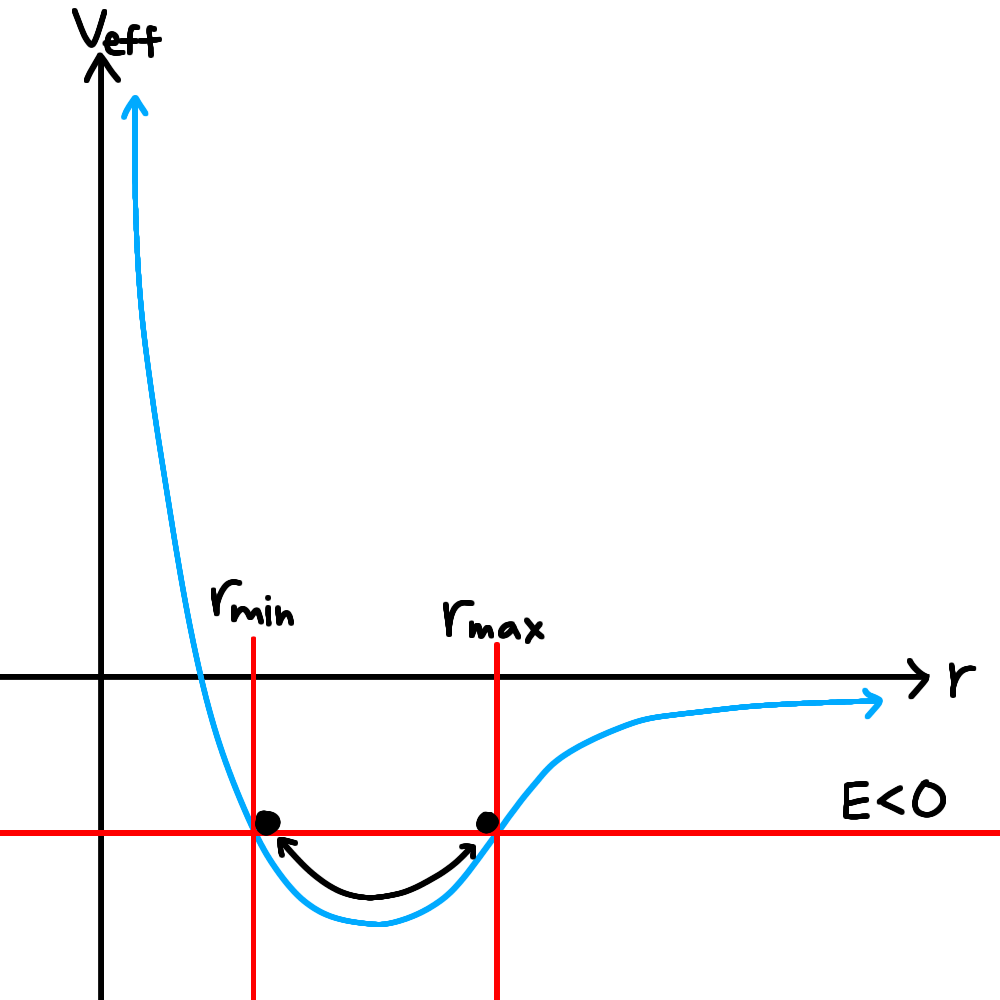
\includegraphics[width=0.8\linewidth]{effective_potential}
  \caption{Effective potential graph.}
  \label{fig:effectivepotential}
\end{minipage}%
\begin{minipage}{.5\textwidth}
  \centering
  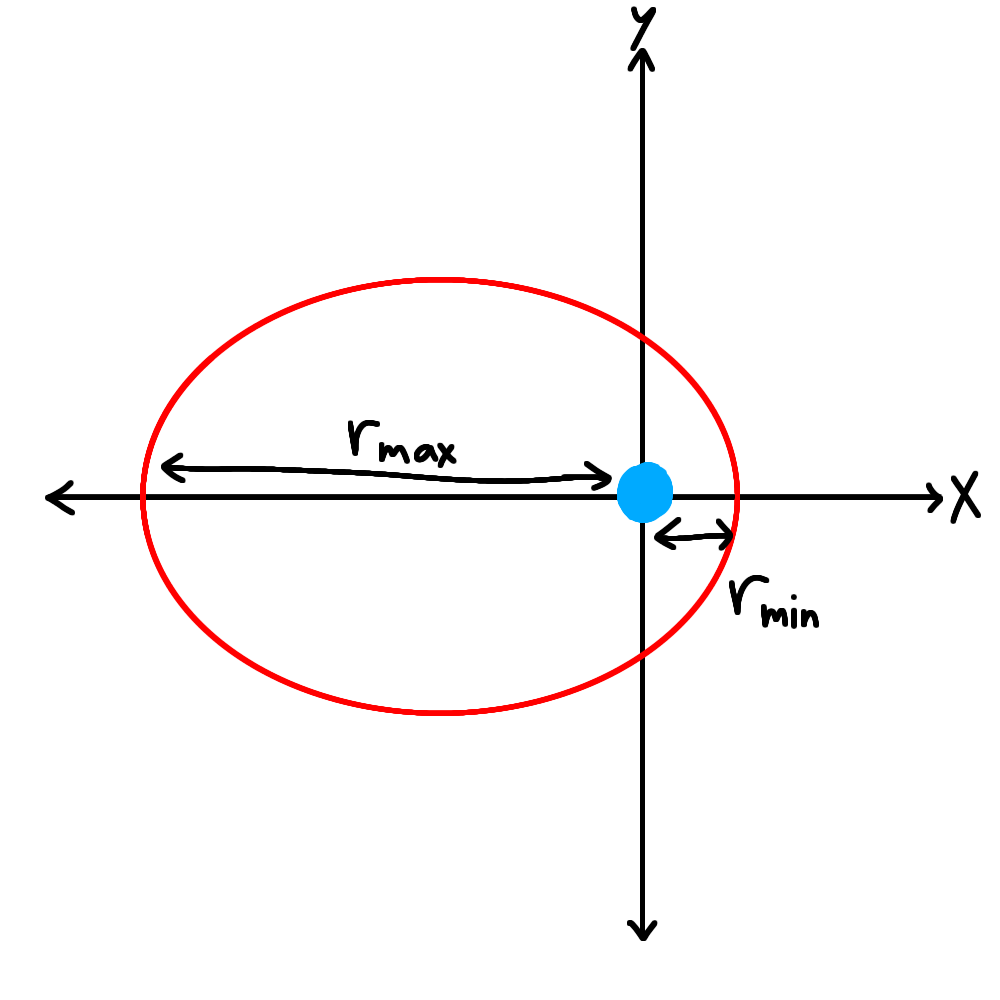
\includegraphics[width=0.8\linewidth]{elliptic_diagram}
  \caption{Diagram of elliptic orbit with large mass $M$ at origin.}
  \label{fig:ellipticdiagram}
\end{minipage}
\end{figure}

When an orbiting mass has an energy $E > 0$, it will orbit in an elliptical orbit.
$r_{\text{min}}$ and $r_{\text{max}}$ are essentially solutions to $E = V_{\text{eff}}(r)$, and therefore where $\dot{r} = 0$.

\[
E = \frac{L^2}{2mr^2} - \frac{GmM}{r}
\]

\[
\text{Solutions: } r_{\text{min}} = a(1 - \epsilon)\text{, } r_{\text{max}} = a(1 + \epsilon)
\]

For negative $E$:

\[
\epsilon = \sqrt{1 + \frac{2EL^2}{m(GmM)^2}}\text{ is eccentricity}
\]

\[
a = -\frac{GmM}{2E}\text{ is the semi-major axis}
\]

\newpage

\subsubsection{Positive energy}

Once $E>0$, $\epsilon$ is still defined in the same way, but there will only be a single solution to the equation because the orbit is unbound.
Because $\epsilon > 1$ when $E>0$, we can also observe that the unbound orbit will be \emph{hyperbolic}.

\begin{figure}[h]
    \centering
    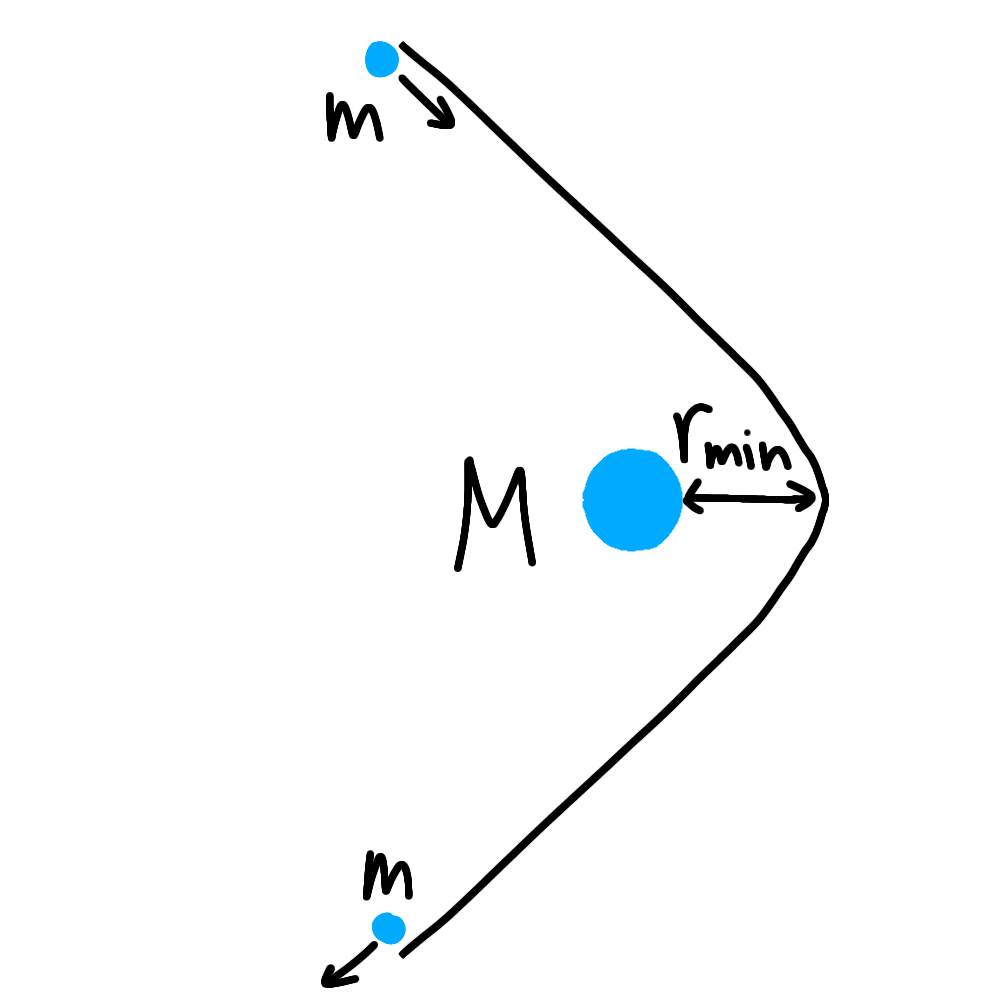
\includegraphics[width=0.35\textwidth]{hyperbolic_orbit}
    \label{fig:hyperbolicorbit}
    \caption{Diagram of a hyperbolic orbit.}
\end{figure}

\subsection{Location labels}

\begin{figure}[h]
    \centering
    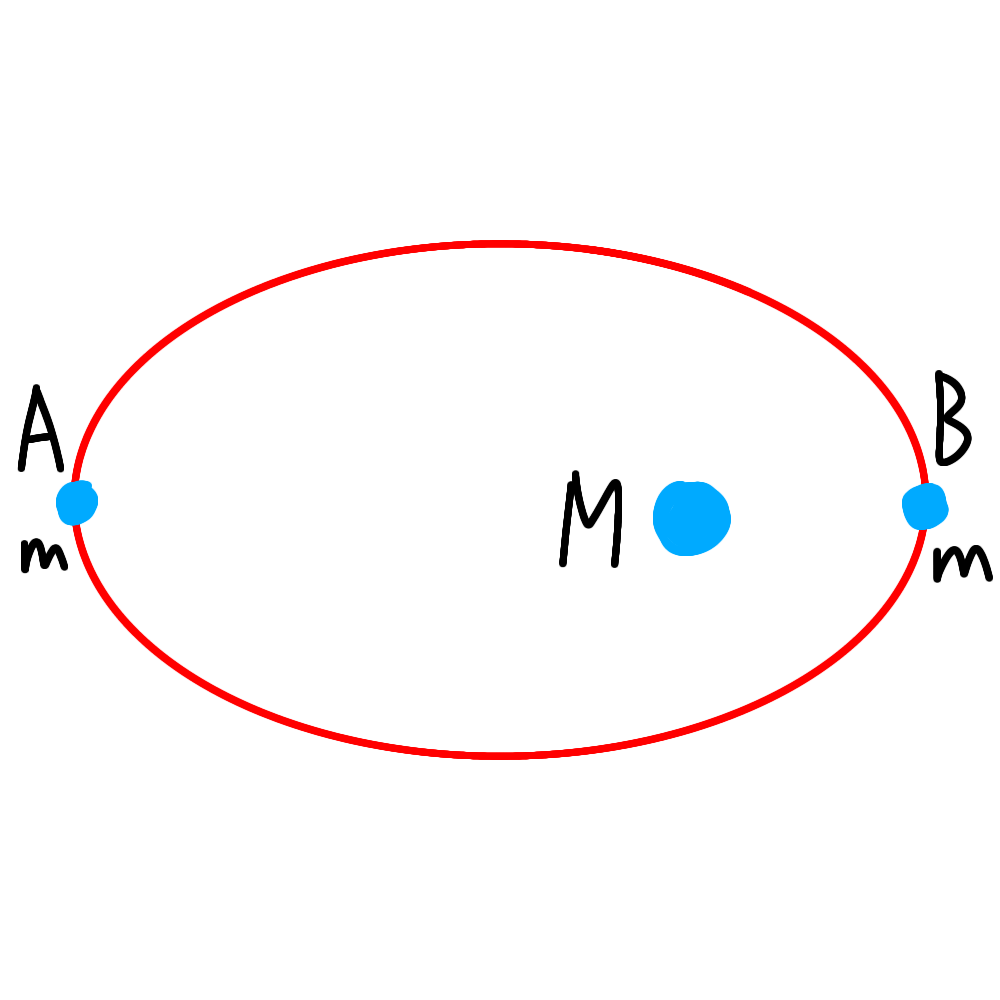
\includegraphics[width=0.35\textwidth]{location_labels}
    \label{fig:locationlabels}
    \caption{Diagram of a locations in elliptic orbit.}
\end{figure}

Considering the situation in Figure \ref{fig:locationlabels}:

\begin{itemize}
	\item When $M$ is the \emph{Sun}, location $A$ is the \emph{aphelion}, and location $B$ is the \emph{perihelion}.
	\item When $M$ is a \emph{star}, location $A$ is the \emph{apastron}, and location $B$ is the \emph{periastron}.
	\item When $M$ is the \emph{Earth}, location $A$ is the \emph{apogee}, and location $B$ is the \emph{perigee}.
\end{itemize}

\end{document}